\section{Field Study}
A small-scale study was conducted which ran for 3 weeks and included 10 participants (including the author). In the study the participants used the application discussed in Chapter \ref{chapter:05-api-implementation} that collected their location data and computed mobility features daily.

% Self-study was conducted first and foremost to evaluate parameters for stops and places
% I have a new phone, app isnt killed there
% Larger study was conducted to validate the package on a broader scale, in contrast to unit testing
% Is it feasible? Is it even possible to track location so frequently, will it die on its own?
% Do they algorithms produce meaningful results
% Tracked for 3 weeks
% Compare answers to computed results
% Try to match time wise as close as possible

\subsection{Self-study}
Before the main study was conducted a self-study was conducted in three different cities, in order to develop the app. Part of the parameter tweaking happened while the author was in Munich where he sat in a large university building and visited different offices. In Figure \ref{fig:tum-map} the Places and the Stops at the university are displayed and as can be seen which are very close. Had the radius parameter for finding places been higher then some the places would have been merged into a single place. Here, the parameter was set to 25 meters, and in the final study it was chosen to set it to 50 meters.

\begin{figure}
    \centering
    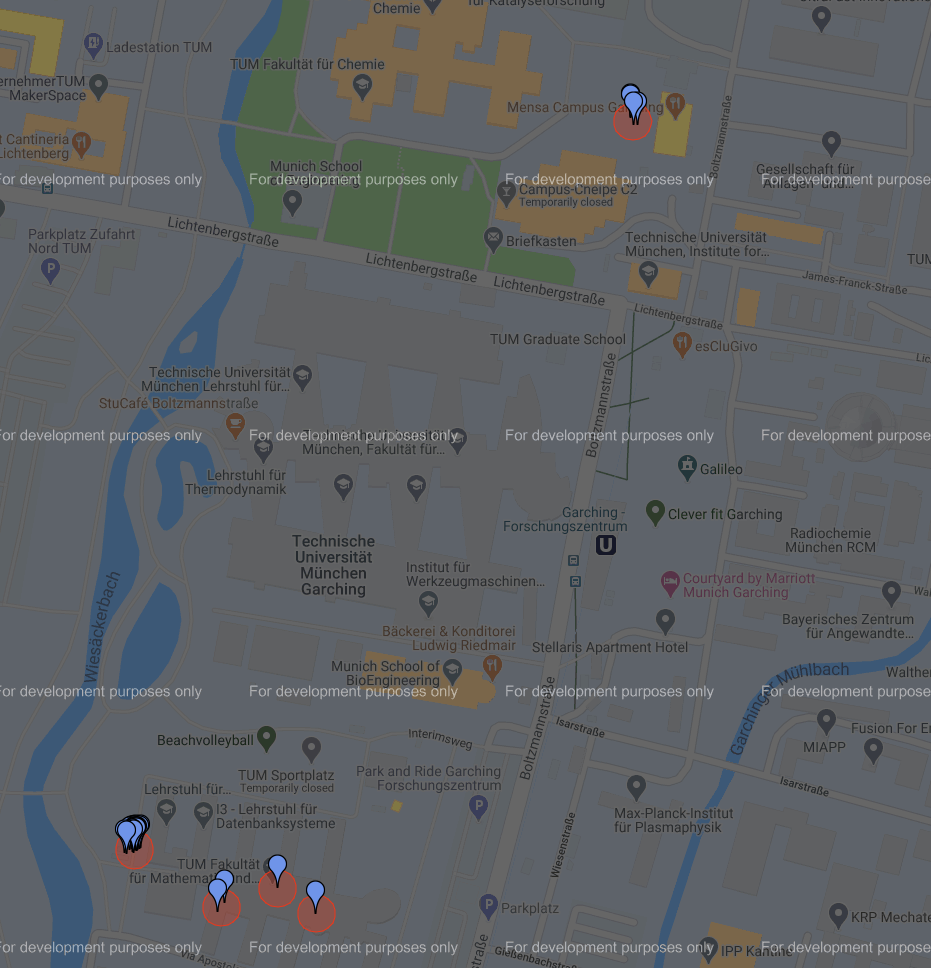
\includegraphics[width=0.7\textwidth]{images/map/map-tum.png}
    \caption{A map of TUM Garching, displaying the Places (red clusters) as well as the Stops which make up these places (blue markers) visited by the author}
    \label{fig:tum-map}
\end{figure}

\subsection{Main Study}
 In addition to this the application also had a diary consisting of 4 questions that the user had to fill out each day. In order to make it easy for the user to remember filling out the diary, a FireBase Cloud Messaging service was created which sent the user a daily notification at 8 PM. The time 8PM was chosen due to being relatively late while still being early enough in the day that people would still be checking their phone. Some people go to bed at 9-10 PM which had to be taken into account. The diary questions were related to 3 of the Mobility Features which were \textit{Number of Clusters}, \textit{Home Stay} and \section{Routine Index}. The point of the questions were to get a subjective estimates of the values of these features. It is important to stress the fact that these these answers are estimates since the user cannot be expected to give very precise answers and secondly they are very subjective since the definition of things such as a 'Place' may vary a lot from person to person.

\subsection{Diary}
Answers were collected through a diary in order to evaluate, to choose the most important parameters certain features were evaluated through comparing subjective answers with calculated features. The features had to be ease to formulate as a question such that subjective user answers could be collected, as such features such as entropy and location variance were ill-suited, whereas Home Stay, Number of Places and Routine Index were chosen instead. 

For collecting the subjective number of places the user was simply asked for the number of places visited today. 

For collecting the subjective home stay percentage, the user was asked the inverse question, i.e. how many hours they were away from their home today. Home Stay feature is calculated including the time spent during the night, and by asking the inverse, one avoids communicating these implementation details to the user. 

The Routine Index was more difficult to formulate as a question, and in the end it was decided upon a scale from 0 to 5, 0 indicating that today looks nothing like previous days and 5 indicating it is exactly the same. Ideally the scale would be more fine grained such as 0 to 10, however this put too much on the user, the main information we wished to draw from the user was a very high level overview of whether the day today was a lot like the previous days.

The questions the user was asked were

\begin{itemize}
    \item[\#1] How many unique places (including home) did you stay at today?
    \item[\#2] How many hours did you spend away from home today? (Rounded-up)
    \item[\#3] Did you spend time at places today that you don't normally visit?
    \item[\#4] On a scale of 0-5, how much did today look like the previous, recent days? (Where 0 means 'not at all' little and 5 means 'Exactly the same')
   
\end{itemize}

Where question \#3 and \#4 relate the routine index feature.

\subsection{The Impact of COVID-19}
The Corona virus pandemic lead to Denmark closing its borders and urging people to stay at home as much as possible. This included workplaces shutting down and people had to work from home, as well as places of recreational character such as gyms and restaurants. This had some major implications for the study and meant that it would be expected that the participants routine was quite steady, since they were mostly home, and that the home stay percentage was very high and that the number of places visited was very low. In addition it was probably also not common for most people go visit new places during the pandemic. However, all in all the pandemic only shaped the results of the field study and did not prevent the study from taking place at all.

\subsection{Data Storage}
To store the data from the study online, such that it could later be extracted for data analysis, a Firebase file storage server was used for uploading files multiple times daily. Concretely, the SingleLocationPoints, Stops and Moves were stored locally on device. Whenever a Feature calculation was triggered, the calculated MobilityContext was serialized and uploaded as a file, in addition to the data points for the day and all Stops and Moves on the phone for the period. This process was very wasteful in the sense that only 'new' data points needed to be uploaded, but instead the whole file was just overwritten. This was mainly done to ensure little data loss and avoid inconsistencies between the online file and the local file.
